\documentclass[11pt]{article}

\usepackage{graphicx} %Required for diagrams
\usepackage[export]{adjustbox} %Required to Adjust Image alignment
\usepackage{float}
\usepackage[bookmarks=true]{hyperref}
\usepackage{bookmark}%Required to do pdf bookmarking
\usepackage{hyperref}%Required for referencing website pages



\begin{document}
\begin{titlepage}
\begin{center}

\includegraphics[width=350px]{University_of_Pretoria_Logo.png}\newline
% Title
\textsc{\LARGE COS301 Mini Project Functional Requirements Specification}\newline


%\begin{minipage}{0.4\textwidth}
\textbf{Group 4B} \\
\begin{flushright} \large
Kyhle Ohlinger \emph{u11131952} \newline
Andrew Parkes \emph{u12189139} \newline
Sifiso Shabangu \emph{u12081622} \newline
New Member \emph{uxxxxxxxx} \newline
New Member \emph{uxxxxxxxx} \newline
New Member \emph{uxxxxxxxx} \newline
New Member \emph{uxxxxxxxx} \newline \newline \newline
\end{flushright}
%\end{minipage}
Here's a link to \href{https://github.com/KyhleOhlinger/COS301-Group-4_B.git}{Github}.


\vfill

{\large Version 1}
\\
{\large \today}

\end{center}
\end{titlepage}


\tableofcontents	%Creates Table of contents from sections and 							 subsections, etc...
\newpage


\section{Introduction}

The purpose of this document is to fully specify and outline the functional requirements of "The use of Online Discussions in Teaching (TODT)" research project, received from the Computer Science Education Didactic and Applications Research (CSEDAR) team, of the Computer Science Department of the University of Pretoria. The document also serves to give the client and developers a clear description and elaboration of the system to be implemented in its totality.

\section{Vision}

The project aims to provide an online space, which will be integrated into the CS website, where students, teaching assistants, and lecturers can engage in activities related to learning the content of specific modules. The system will also apply game-like concepts to motivate students to increase the quality of their participation, and consequently experience a deeper understanding of the course content.

\section{Background and System Description}

This project is due to the Computer Science department of the University of Pretoria having problems with the currently available tools for discussion forums. The following problems are hampering positive engagement of both teaching staff and students:
\begin{itemize}
\item Unorganised content,
\item User Inexperience, and 
\item Low levels of excitement.
\end{itemize}
The System intends to create an online discussion forum that has automated feedback on common mistakes, game-like presention as well as automated structuring. \newline
The system also provides the COS 301 students with the opportunity to learn about the procedures used for creating, designing and developing projects for businesses, while also providing the University of Pretoria with a potentially new system that may be released as an opensource project, that could possibly be implemented worldwide.
\subsection{Related Project}
The project is a face lift to the existing discussion forum of the Department of Computer Sciences, and aims to improve the existing one by bringing new features that would encourage students to be more involved in discussing certain modules.
\subsection{System Environment}
The system will interact with LDAP ,which will handle credentials avoiding the need for a database.

\section{The Stakeholders}

\subsection{The Client}
The Client is Ms Vreda Pieterse at the Department of Computer Science.
\subsection{The customers}
The Customers are Students of the Computer science who are enrolled in the modules, and lectures in the department.
\subsection{Maintenance Users}
The system will be assigned administrators from the Computer Science department and they will ensure its maintenance.

\newpage
\section{Functional Requirements}
\subsection{Scope and Limitations/Exclusions}
\textbf{Scope: } \newline
The scope of the Buzz System project can be encapsulated as a solution that allows the users of the system to:
\begin{itemize}
\item Have access to basic the functionalities that are common on all online forums.
\item The administrative staff should be able to manage the registration of users to the forum.
\item User has to be able to participate in discussions. 
\end{itemize}
The system shall be designed primarily for use by lecturers, teaching
assistants, and students for the core purpose of engaging in activities related to learning the content of specific modules, and increasing the participation, and consequently deeper understanding of the modules at hand. \newline
\textbf{Limitations/Exclusions: } \newline

\subsection{Required Functionality}
The following system processes describe the functional requirements of the system.
\begin{enumerate}
\item CRUD Operations:
	\begin{itemize}
	\item \textbf{Purpose:}
	Users should be able to create, read, update and delete posts.
	\newline
	\textbf{Limitations:} Not all users should be able to use all the functions. Some users may even CRUD other users posts.
	\item \textbf{Importance: } Critical
	\item \textbf{Pre-Conditions: }
		\begin{itemize}
		\item Buzz space must exist.
		\item User must be connected to the buzz system.\item 	
		
		\textit{Create: }
			\begin{itemize}
    			\item Must have necessary permission to create posts.
    			\item Must be registered on the buzz system.
  			\end{itemize}
  			
		\item \textit{Read: }
			\begin{itemize}
			\item Post must exist.
			\end{itemize}
	
		\item \textit{Update: }
			\begin{itemize}
			\item Post must exist.
			\item Must either be owner of the post, or have necessary 				permissions to update the post.
			\end{itemize}

		\item \textit{Delete: }
			\begin{itemize}
			\item Post must exist.
			\item Must either be owner of the post, or have necessary 				permissions to delete the post
			\end{itemize}  			
  			
		\end{itemize}
		\item \textbf{Post-Conditions: }
		\begin{itemize}
		\item \textit{Create: }
			\begin{itemize}
			\item Post will have been created.
			\item Post may not have been created, due to some error.
			\end{itemize}
		\item \textit{Read: }
			\begin{itemize}
			\item If logged in, post will be marked as read for the 				specific user.
			\end{itemize}
		\item \textit{Update: }
			\begin{itemize}
			\item Post will be updated if user has required 						permissions.
			\item Post may not have been updated due to some error.
			\end{itemize}
		\item \textit{Delete: }
			\begin{itemize}
			\item Post will be marked as deleted, and thus removed 					from the discussion board.
			\item Post is not actually removed from the server, it is 					however hidden from all users.
		\item Post may not have been deleted due to some error. 
			\end{itemize}			
			
		\end{itemize}
	
	\end{itemize}
	
\item Tracking read and unread messages:
\begin{itemize}
\item 
\textbf{Purpose:}
The system must keep track of who has read what, and highlight unread messages for each user.
\newline

\item \textbf{Importance:} Critical
\item \textbf{Pre-Conditions: }
	\begin{itemize}
	\item Buzz space must exist.
	\item User must be registered to the buzz system.
	\item User must be logged into the system while viewing the post.
	\end{itemize}

\textbf{Post-Conditions: }
	\begin{itemize}
	\item Post is marked as read.
	\item Post remains unmarked due to some error.
	\end{itemize}

\end{itemize}


\item Message Restrictions: 
\begin{itemize}
\item \textbf{Purpose:}
This deals with the restriction of posting messages.
\newline
\textbf{Limitations:} 
Message length should be restricted. Content type should also be restricted based on level and status of the user posting the message.

\item \textbf{Importance:} Critical\newline
\textbf{Pre-Conditions: }
	\begin{itemize}
	\item Buzz space must exist.
	\item User must be registered to the buzz system.
	\item User must have necessary permissions to create posts of a 		certain length or content type.
	\item Content type and message length must be established by the 		creator of that specific buzz (configurable).
	\end{itemize}

\textbf{Post-Conditions: }
	\begin{itemize}
	\item Post is created.
	\item Post may not have been created due to some error.
	\end{itemize}
\end{itemize}


\item Social Tagging 
\begin{itemize}
\item \textbf{Purpose:}
This deals with social tagging, broad folksnomy type is used
in this social tagging
\newline
\textbf{Limitations:} 
Not all users will be able to tag a buzz
space, Users with higher privileges and lectures will be able to social
tag buzz space

\item \textbf{Importance:} Critical\newline
\textbf{Pre-Conditions: }
	\begin{itemize}
	\item Buzz space must exist.
	\item User must be registered to the buzz system.
	\item Buzz space must have a rating from users to be tagged .
	\end{itemize}

\textbf{Post-Conditions: }
	\begin{itemize}
	\item Buzz space tagged with a keyword.
	\item Buzz space available at tag box for fast access.
	\end{itemize}
\end{itemize}

\item Self organise
\begin{itemize}
\item \textbf{Purpose:}
TThis deals with self-organisation based on social tagging and
allow the user to view according to the base structure, owns structure
or public structure.
\newline
\textbf{Limitations:} 
Users with higher privileges will be able to
organise view to their own structure.

\item \textbf{Importance:} Critical\newline
\textbf{Pre-Conditions: }
	\begin{itemize}
	\item Buzz space must exist.
	\item User must be registered to the buzz system.
	\item Buzz space must have a rating from users to be tagged .
	\item Social tagging must be applied to other buzz space
	\end{itemize}

\textbf{Post-Conditions: }
	\begin{itemize}
	\item Tagged buzz space with higher rating from users will be organised
to be in base structure
	\item Most accessed tagged buzz space will be included in public struc-
ture.
	\item Users with buzz space can organise their own structure.
	\end{itemize}
\end{itemize}

\item Buzz Tag
\begin{itemize}
\item \textbf{Purpose:}
This deals with an addition of a read later section, which saves
buzz space with long comments for a user to read later when logged
in and remind the user every time when logged.
\newline
\textbf{Limitations:} 
All users will have this feature by default

\item \textbf{Importance:} Critical\newline
\textbf{Pre-Conditions: }
	\begin{itemize}
	\item Buzz space must exist.
	\item User must be registered to the buzz system.

	\end{itemize}

\textbf{Post-Conditions: }
	\begin{itemize}
	\item Read later section will be created and added on the side of the
users portal
	\item Buzz space reference must be saved in a read later section on the
user’s portal is the user clicked a buzz space to read later section
	
	\end{itemize}
\end{itemize}

\item Read Later Section
\begin{itemize}
\item \textbf{Purpose:}
This deals with buzz space tagging for least privilege users
,this will help social tagging by providing trending buzz space and
notification system for users who opened buzz space or waiting for a
reply on a comment.
\newline
\textbf{Limitations:} 
All users will have this feature by default

\item \textbf{Importance:} Critical\newline
\textbf{Pre-Conditions: }
	\begin{itemize}
	\item Buzz space must exist.
	\item User must be registered to the buzz system.
	\item User optioned for notifications when registering on the buzz sys-
tem

	\end{itemize}

\textbf{Post-Conditions: }
	\begin{itemize}
	\item Menu will be provided to the user with icons similar to Glyphicons
to describe the buzz space thread for the user to click on.
	\item After user click a certain icon , thread will be rated according to
the icon and each icon have description of the buzz space thread
ranging from lame buzz thread space to must read buzz thread
space and also apply to comments on the buzz space thread .
\item Notification will be send atomically to users read later section to
inform about a new comment on the buzz space user commented
	
	\end{itemize}
\end{itemize}


\end{enumerate}




\subsection{Use case Prioritization}
\begin{itemize}
\item \textbf{Critical: }
	\begin{itemize}
		\item CRUD operations.
		\item Tracking read and unread messages.
		\item Message Restrictions.
	\end{itemize}

\item \textbf{Important: }
	\begin{itemize}
		\item ...
	\end{itemize}

\item \textbf{Nice-to-Have: }
	\begin{itemize}
		\item Social Tagging
		\item Self organise
		\item Buzz Tag
		\item Read Later Section
	\end{itemize}
\end{itemize}
\subsection{Use case/Services Contracts}
Temporary words
\subsection{Process Specifications}
Temporary words
\subsection{Domain Model}
Temporary words

\newpage
\section{Temporary Space}

\subsection{Andrew}



\newpage

\subsection{Sifiso}
\subsubsection{Point 1:} 
\begin{enumerate}
\item 
\textbf{Scope:}
This deals with social tagging, broad folksnomy type is used in this social tagging
\newline
\textbf{Limitations/exclusions:} 
Not all users will be able to tag a buzz space, Users with higher privileges and lectures will be able to social tag buzz space

\item 
\textbf{Use case Prioritization:} nice to have

\item 
\textbf{Use case/Service Contracts:} 
\newline
\textbf{Pre-Conditions: }
\begin{itemize}
\item User must be registered to the buzz system.
\item User must have necessary privileges.
\item Buzz space must have a rating from users to be tagged
\end{itemize}
 

\textbf{Post-Conditions: }
\begin{itemize}
\item Buzz space tagged with a keyword.
\item Buzz space available at tag box for fast access.
\end{itemize}
\end{enumerate}

\subsubsection{Point 2:} 
\begin{enumerate}
\item 
\textbf{Scope:}
This deals with self-organisation based on social tagging and allow the user to view according to the base structure, owns structure or public structure.
\newline
\textbf{Limitations/exclusions:} 
Users with higher privileges will be able to organise view to their own structure.
\item 
\textbf{Use case Prioritization:} nice to have

\item 
\textbf{Use case/Service Contracts:} 
\newline
\textbf{Pre-Conditions: }
\begin{itemize}
\item User must be registered to the buzz system.
\item User must have necessary privileges.
\item Buzz space must have a rating from users.
\item Social tagging must be applied to other buzz space
\end{itemize}
 

\textbf{Post-Conditions: }
\begin{itemize}
\item Tagged buzz space with higher rating from users will be organised to be in base structure
\item Most accessed tagged buzz space will be included in public structure.
\item Users with buzz space can organise their own structure.
\end{itemize}
\end{enumerate}

\subsubsection{Point 3:} 
\begin{enumerate}
\item 
\textbf{Scope:}
This deals with an addition of a read later section, which saves buzz space with long comments for a user to read later when logged in and remind the user every time when logged.
\newline
\textbf{Limitations/exclusions:} 
All users will have this feature by default
\item 
\textbf{Use case Prioritization:} nice to have

\item 
\textbf{Use case/Service Contracts:} 
\newline
\textbf{Pre-Conditions: }
\begin{itemize}
\item User must be registered to the buzz system.
\end{itemize}
 

\textbf{Post-Conditions: }
\begin{itemize}
\item Read later section will be created and added on the side of the users portal
\item Buzz space reference must be saved in a read later section on the user's portal is the user clicked a buzz space to read later section 
\end{itemize}
\end{enumerate}

\subsubsection{Point 4:} 
\begin{enumerate}
\item 
\textbf{Scope:}
This deals with buzz space tagging for least privilege users ,this will help social tagging by providing trending buzz space and notification system for users who opened buzz space or waiting for a reply on a comment.
\newline
\textbf{Limitations/exclusions:} 
All users will have this feature by default
\item 
\textbf{Use case Prioritization:} nice to have

\item 
\textbf{Use case/Service Contracts:} 
\newline
\textbf{Pre-Conditions: }
\begin{itemize}
\item User must be registered to the buzz system.
\item User must be allowed to the buzz space.
\item User optioned for notifications when registering on the buzz system

\end{itemize}
 

\textbf{Post-Conditions: }
\begin{itemize}
\item Menu will be provided to the user with icons similar to Glyphicons to describe the buzz space thread for the user to click on.
\item After user click a certain icon , thread will be rated according to the icon and each icon have description of the buzz space thread ranging from lame buzz thread space to must read buzz thread space and also apply to comments on the buzz space thread .
\item Notification will be send atomically to users read later section to inform about a new comment on the buzz space user commented 
\end{itemize}
\end{enumerate}



\newpage

\subsection{Maret}

\subsubsection{Point 1:}
\begin{enumerate}
\item 
\textbf{Scope}
 The system must send template messages automatically to individual users or specified groups, like a welcomming message or a notification message.
\newline
\textbf{Limitations/exclusions:}
\item
\textbf{Use case Prioritization:} Nice-to-have
\textbf{Use case/Service Contracts:} 
\newline
\textbf{Pre-Conditions: }
\begin{itemize}
\item The user must be registered to the buzz system.
\item The message template should exist.
\item The system must be able to select a cetain group based on specific information, to send the group message to.
\end{itemize}
 \textbf{Post-Conditions: }
\begin{itemize}
\item The user must be alerted of the message.
\item The user must not be albe to reply to the message.
\item The user must be able to delete the messages.
\item The user must not be able to see what other users have received the same message via group messaging.
\end{itemize}
\end{enumerate}

\subsubsection{Point 2:}
\begin{enumerate}
\item 
\textbf{Scope}
The system must automatically change the status of a user based on his participation.
\newline
\textbf{Limitations/exclusions:}
\item
\textbf{Use case Prioritization:} Important
\textbf{Use case/Service Contracts:} 
\newline
\textbf{Pre-Conditions: }
\begin{itemize}
\item The user must be registered to the buzz system.
\item The user must be logged in for his status to be affected by his participation.
\item The users current status will be updated, so he must have a current status.
\end{itemize}
 \textbf{Post-Conditions: }
\begin{itemize}
\item The users privileges change when his status change.
\item The user must be able to view his status.
\item The users stutus is public.
\end{itemize}
\end{enumerate}


\subsection{Matthew}
\subsubsection{Point 1:}
\begin{enumerate}
\item 
\textbf{Scope:}
Statistical information created from evaluation to capture average mark of every student within a time frame. Visual reporting of a participants evaluation in correlation to the average of the evaluation of all users or certain groups of users for gamification concept.
\newline
\textbf{Limitations/exclusions:} : Not all users may see statistical information of users. Only higher level users may view statistical information and visual reporting of users.

\item 
\textbf{Use case Prioritization:} Important.

\item 
\textbf{Use case/Service Contracts:} 

\textbf{Pre-Conditions: }
\begin{itemize}
\item User must be connected to buzz.

\item User must be part of discussion or module to be evaluated.

\item User may not be of higher level of the users who monitor the statistical information.


\end{itemize}
 

\textbf{Post-Conditions: }
\begin{itemize}

\item Results and statistical information may not be altered.
\item No more statistical information may be formulated once time period passes.
\item All users may see there statistical information.
\item Statistical information will be represented in a visual representation from that time period.



\end{itemize}
\end{enumerate}

\subsubsection{Point 2:} 
\begin{enumerate}
\item 
\textbf{Scope:}
Improved post editor for example text formatting and automatic pretty printing of code in posts.
\newline
\textbf{Limitations/exclusions:} 

Not all users will be able to use these options. Has to be earned. Certain options are available for all users by default.

\item 
\textbf{Use case Prioritization:} Nice-To-Have.

\item 
\textbf{Use case/Service Contracts:} 
\newline
\textbf{Pre-Conditions: }
\begin{itemize}
\item User must be connected to buzz system.
\item User must be of a high enough level.
\item Users must be using the post editor.
\end{itemize}
 

\textbf{Post-Conditions: }
\begin{itemize}

\item Message will be formatted accordingly and marked up (e.g. font colouring,emoticons,various fonts)to how the user wanted. 
\item User must send message to be viewable by other users.
\end{itemize}
\end{enumerate}

\subsection{Sphelele}
\subsubsection{Point 1: }
\begin{enumerate}
\item \textbf{Scope: }
The website will allow users to search the website for topics and buzz spaces, and then filter those search results by various categories. \newline \newline
	  \textbf{Limitation/Exclusions: }
Users will be limited to 4 filter categories, namely: topic, date posted/last updated, buzz space name and rating.
\item \textbf{Use case Prioritization: } Important
\item \textbf{Use case/Service Contracts: } \newline \newline
	  \textbf{Post-Conditions: }
	  \begin{itemize}
	  \item Search results are returned
	  \item	Search filters are successfully executed
	  \end{itemize}
	  \item
	  \item
	  \item
	  \end{enumerate}
	  
	  \subsubsection{Point 2:}
	  \begin{enumerate}
	  
	  
	  \item \textbf{Scope:} The website will allow users to evaluate/vote for posts on the website. \newline \newline
	  \textbf{Limitations/Exclusions:} Only users that are logged in to the system and have the privilege rights to evaluate/vote on posts will be allowed to evaluate/vote on posts. Higher Privileged users' votes will push posts higher (or lower) than lower privileged users. \newline \newline
	  
	  \item \textbf{Use case Prioritization: } Important \newline \newline
	  \item \textbf{Use Case/Service Contract: } \newline \newline
	  \textbf{Pre-Conditions}
	  \begin{itemize}
	  
	  \item User privilege level allows user to vote for post
	  \item post must exist and not be removed
	  \end{itemize}
	  \textbf{Post Conditions}
	  \begin{itemize}
	  \item Post rating is updated.
	  \item post moves up/down accordingly
	  \end{itemize}
	  \item
	  \item
	  \item
	  \end{enumerate}

\newpage

\graphicspath{ {../Diagrams/Tienie/Plagiarism/} }

\subsection{Tienie}
\subsubsection{Point 1: }
\begin{enumerate}
\item \textbf{Scope: }
This deals with the built in plagiarism checker. It describes the functionality of the plagiarism checker as well as its aims and goals.
\newline
\textbf{Limitations/exclusions:} 
The plagiarism checker is built into the system, and is thus not an optional feature for users posting. However, the checker may be configurable (i.e. turned on and off) by board administrators.
\item 	\textbf{Use case Prioritization: } Nice-To-Have
\item 	\textbf{Use case/Service Contracts: }
		\begin{itemize}
			\item	\textbf{Pre-Conditions}
			\begin{itemize}
	  			\item All posts from within the website will need to be available for traversal in text format.
	  			\item A reference collection of documents assumed to be valid will need to be obtained for traversal in text format.
	  			\item A similarity threshold will need to be agreed upon.
	  			\item Access to the Internet (not just Intranet) is a must.
	  			\item A google Search Engine ID and API Key for getting RESTful results to get web search results for comparison in JSON format (Google Custom Search Engine – 100 Free Search Queries Per Day)
	  		\end{itemize}
	  		\item	\textbf{Post-Conditions}
	  		\begin{itemize}
	  			\item A moderator must be alerted if the plagiarism percentage surpasses the allowed threshold.
	  			\item The percentage of plagiarism detected must be alerted to a moderator if it surpasses the threshold.
	  			\item If plagiarism is detected above the allowed threshold, the post must be highlighted as suspicious.
	  			\item Unique documents scanned must be added to the repository of reference documents.
	  		\end{itemize}
	  		\newpage
	  		\item	\textbf{Request and Results Data Structures}
	  		\begin{figure}[H]
    			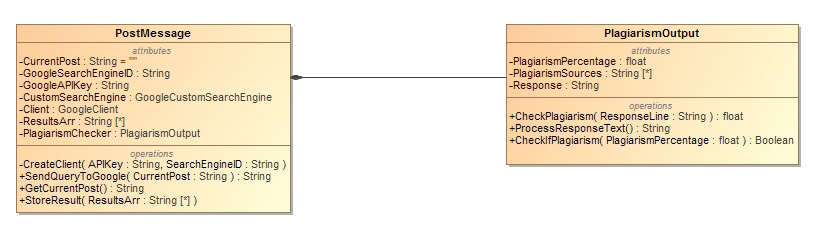
\includegraphics[scale=0.5]{InputOutput.jpg}
			\end{figure}
	  	\end{itemize}
\item	\textbf{Required Functionality}
	\begin{figure}[H]
    	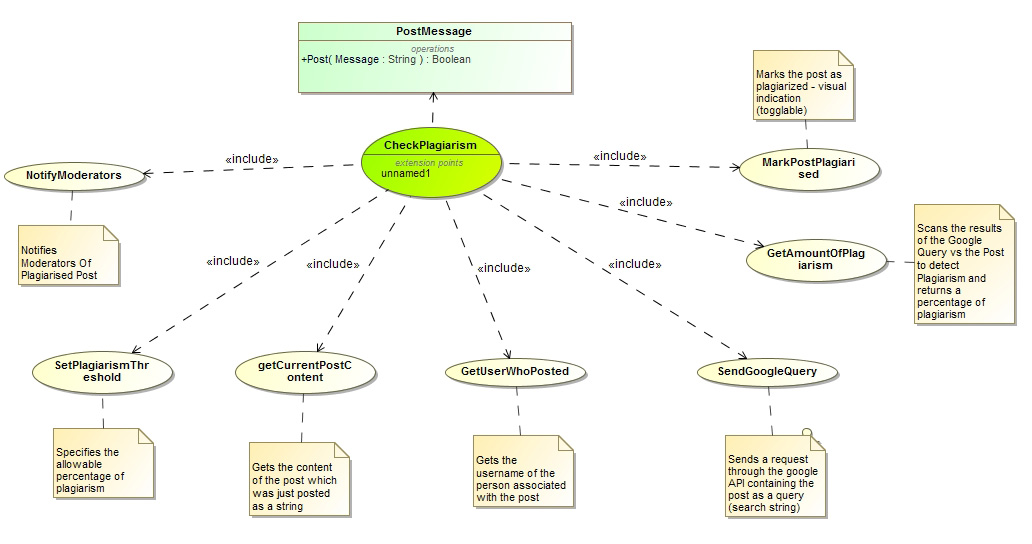
\includegraphics[scale=0.4]{UseCase.jpg}
	\end{figure}
\newpage
\item \textbf{Process Specifications}
	\begin{figure}[H]
    	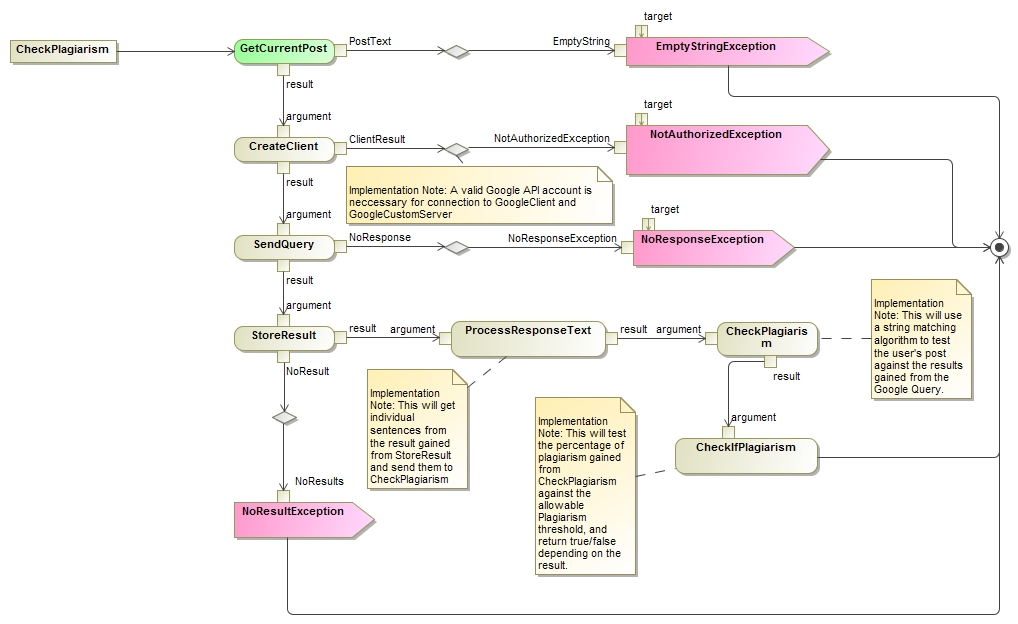
\includegraphics[scale=0.4]{Activity.jpg}
	\end{figure}
	  		
\end{enumerate}
\graphicspath{ {../Diagrams/Tienie/Netiquette/} }
\newpage
\subsubsection{Point 2: }
\begin{enumerate}
\item \textbf{Scope: }
This deals with the built in Netiquette checker. It describes the functionality of the Netiquette checker as well as its aims and goals.
\newline
\textbf{Limitations/exclusions:} 
The netiquette checker is built into the system, and is thus not an optional feature for users posting. However, the checker may be configurable (i.e. turned on and off) by board administrators.
\item 	\textbf{Use case Prioritization: } Nice-To-Have
\item 	\textbf{Use case/Service Contracts: }
		\begin{itemize}
			\item	\textbf{Pre-Conditions}
			\begin{itemize}
	  			\item All posts from within the website will need to be available for traversal in text format
	  			\item The netiquette checker will only check the following netiquette rules:
	  			\begin{itemize}
	  				\item Proper Spelling
	  				\item Repetition of Asked Questions
	  				\item Checking all caps
	  				\item Curse word checking
	  				\item Checking for general insults
	  			\end{itemize}
	  			\item We will need a text file containing a large list of commonly used words for the spell checker.
	  			\item We will need a text file containing a large list of commonly used curse words.
	  			\item We will need a text file containing a large list of words commonly used with the intention of insulting someone.
	  		\end{itemize}
	  		\item	\textbf{Post-Conditions}
	  		\begin{itemize}
	  			\item A moderator must be alerted if a post is detected as violating netiquette.
	  			\item The post must be highlighted to show that it violates netiquette rules.
	  			\item A moderator should be able to hide a post which violates netiquette.
	  			\item The system itself must alert the user of what netiquette rules they have violated as well as give them the opportunity to edit the post and fix them.
	  		\end{itemize}
	  		\newpage
	  		\item	\textbf{Request and Results Data Structures}
	  		\begin{figure}[H]
	  			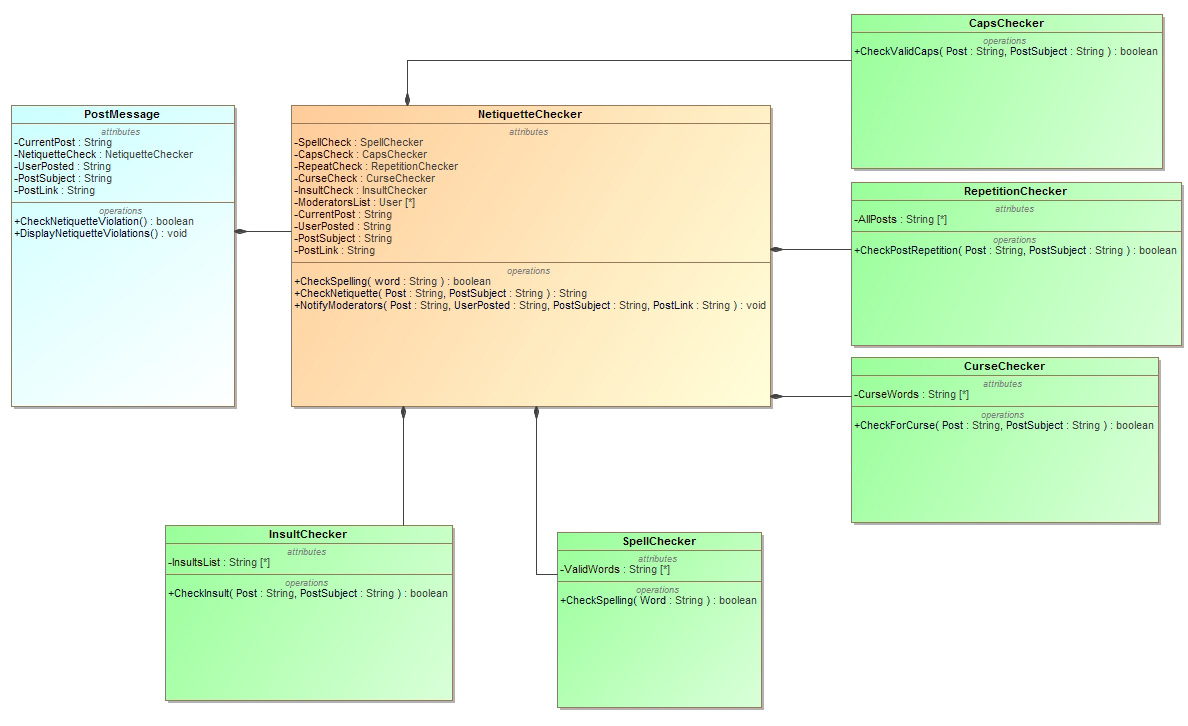
\includegraphics[scale=0.35]{NetInputOutput.jpg}
	  		\end{figure}
	  	\end{itemize}
	  	\newpage
\item	\textbf{Required Functionality}
	  		\begin{figure}[H]
	  			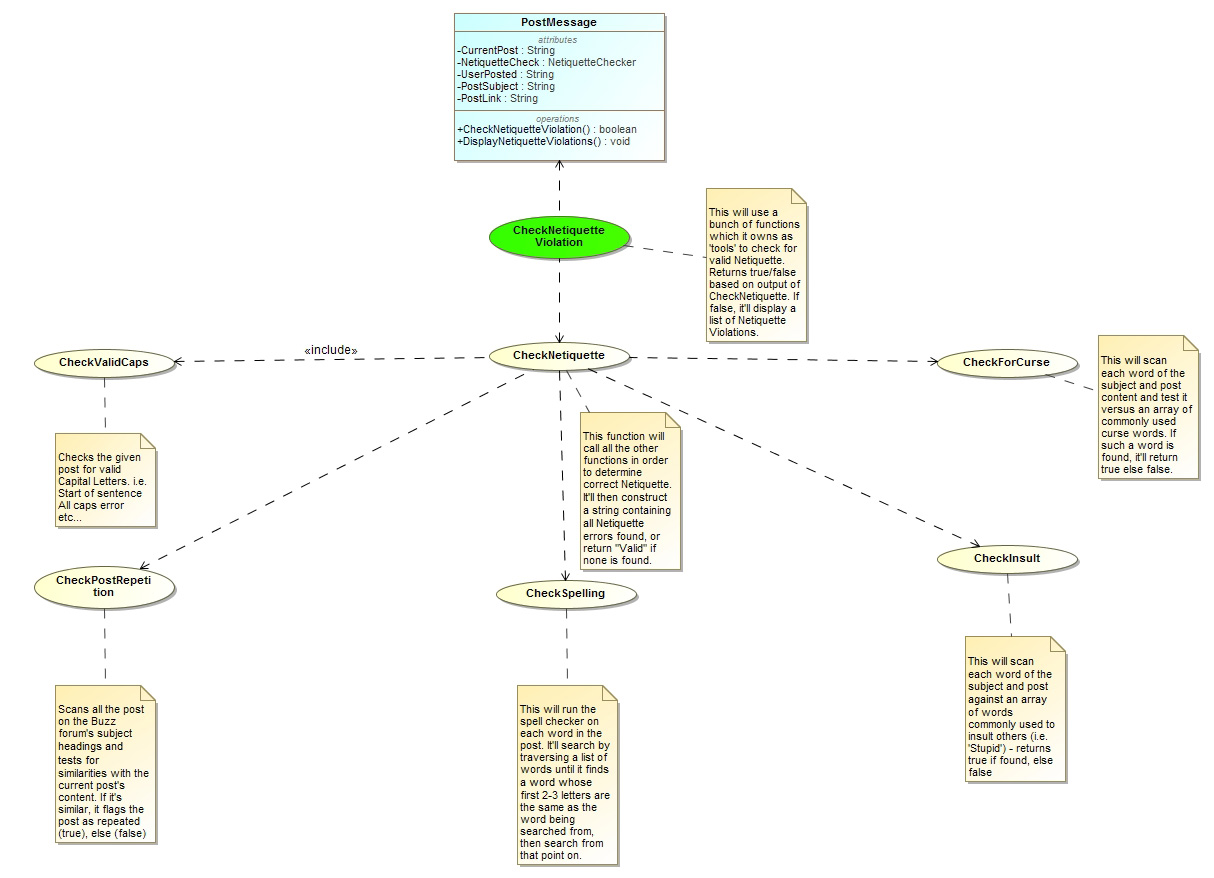
\includegraphics[scale=0.35]{NetUseCase.jpg}
	  		\end{figure}
	  		\newpage
\item \textbf{Process Specifications}
	  		\begin{figure}[H]
	  			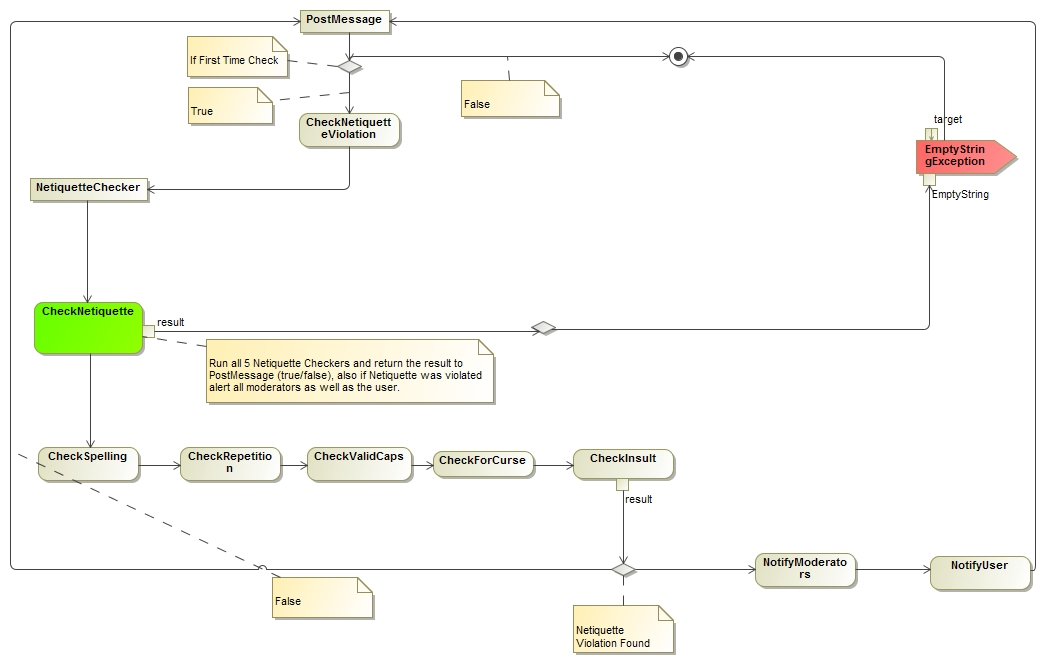
\includegraphics[scale=0.40]{NetProcessDiagram.jpg}
	  		\end{figure}
\end{enumerate}

\newpage

\subsection{name}
\begin{enumerate}
\item 
\item 
\item 
\item 
\item 
\item 
\end{enumerate}

\newpage

\end{document}
